\ifdefined\maindoc\else
% typesetting this chapter as a standalone document
\def\doctitle{Supporting classes}
% starting definitions for both the main document and stand-alone chapters
\documentclass{book}

\def\mech{artisynth.core.mechmodels}
\def\mgeo{maspack.geometry}

% Add search paths for input files
\makeatletter
\def\input@path{{../}{../../}{../texinputs/}}
\makeatother

\usepackage{amsmath}
\usepackage{framed}
%%
%% Default settings for artisynth
%%
\NeedsTeXFormat{LaTeX2e}
%%\ProvidesPackage{artisynthDoc}[2012/04/05]

\usepackage[T1]{fontenc}
\usepackage[latin1]{inputenc}
\usepackage{listings}
\usepackage{makeidx}
\usepackage{latexml}
\usepackage{graphicx}
\usepackage{framed}
\usepackage{booktabs}
\usepackage{color}

\newcommand{\pubdate}{\today}
\newcommand{\setpubdate}[1]{\renewcommand{\pubdate}{#1}}
\newcommand{\code}[1]{{\tt #1}}

\iflatexml
\usepackage{hyperref}
\setlength\parindent{0pt} 
\else
%% then we are making a PDF, so include things that LaTeXML can't handle: 
%% docbook style, \RaggedRight
\usepackage{ifxetex}
\usepackage{xstring}
\usepackage{pslatex} % fixes fonts; in particular sets a better-fitting \tt font

\usepackage[most]{tcolorbox}
\definecolor{shadecolor}{rgb}{0.95,0.95,0.95}
\tcbset{
    frame code={}
    center title,
    left=0pt,
    right=0pt,
    top=0pt,
    bottom=0pt,
    colback=shadecolor,
    colframe=white,
    width=\dimexpr\textwidth\relax,
    enlarge left by=0mm,
    boxsep=0pt,
    arc=0pt,outer arc=0pt,
}%

\usepackage[A4]{artisynth_papersize}
%\usepackage[letter]{artisynth_papersize}
\usepackage[hyperlink]{asciidoc-dblatex} 

%\usepackage{verbatim}
\usepackage{ragged2e}
\setlength{\RaggedRightRightskip}{0pt plus 4em}
\RaggedRight
\renewcommand{\DBKpubdate}{\pubdate}
\renewcommand{\DBKreleaseinfo}{}
\fi

% set hypertext links to be dark blue:
\definecolor{darkblue}{rgb}{0,0,0.8}
\definecolor{sidebar}{rgb}{0.5,0.5,0.7}
\hypersetup{colorlinks=true,urlcolor=darkblue,linkcolor=darkblue,breaklinks=true}

%%%%%%%%%%%%%%%%%%%%%%%%%%%%%%%%%%%%%%%%%%%%%%%%%%%%%%%%%%%%%%%%%%%%%%%%%%%%%
%
% Define macros for handling javadoc class and method references
%
%%%%%%%%%%%%%%%%%%%%%%%%%%%%%%%%%%%%%%%%%%%%%%%%%%%%%%%%%%%%%%%%%%%%%%%%%%%%%
\makeatletter

% macro to enable line break if inside a PDF file
\def\pdfbreak{\iflatexml\else\\\fi}

% code inspired by http://stackoverflow.com/questions/2457780/latex-apply-an-operation-to-every-character-in-a-string
\def\removeargs #1{\doremoveargs#1$\wholeString\unskip}
\def\doremoveargs#1#2\wholeString{\if#1$%
\else\if#1({()}\else{#1}\taketherest#2\fi\fi}
\def\taketherest#1\fi
{\fi \doremoveargs#1\wholeString}

% Note: still doesn't work properly when called on macro output ...
% i.e., \dottoslash{\concatnames{model}{base}{foo}} fails 
\def\dottoslash #1{\dodottoslash#1$\wholeString\unskip}
\def\dodottoslash#1#2\wholeString{\if#1$%
\else\if#1.{/}\else{#1}\fi\dottaketherest#2\fi}
\def\dottaketherest#1\fi{\fi \dodottoslash#1\wholeString}

\def\hashtodot #1{\dohashtodot#1$\wholeString\unskip}
\def\dohashtodot#1#2\wholeString{\if#1$X%
\else\if#1\#{.}\else{#1}\fi\hashtaketherest#2\fi}
\def\hashtaketherest#1\fi{\fi \dohashtodot#1\wholeString}

%\dollartodot{#1} does the same thing as \StrSubstitute[0]{#1}{\$}{.}
% from the packahe xstring. We define \dollartodot instead because
% LaTeXML does not implement xstring.
%
% Note that for the substituion to work, we need \ifx instead of \if,
% since otherwise escaped characters won't work properly:
% if #1 = \$, then \if#1* seems to compare '\' and '$' (and output '*'),
% rather than comparing '$' to '*'
\def\dollartodot #1{\dodollartodot#1*\wholeString\unskip}
\def\dodollartodot#1#2\wholeString{\ifx#1*%
\else \ifx#1\${.}\else{#1}\fi\dollartaketherest#2\fi}
\def\dollartaketherest#1\fi{\fi \dodollartodot#1\wholeString}

% concatenates up to three class/method names together, adding '.' characters
% between them. The first and/or second argument may be empty, in which case
% the '.' is omitted. To check to see if these arguments are empty, we
% use a contruction '\if#1@@', which will return true iff #1 is empty
% (on the assumption that #1 will not contain a '@' character).
\def\concatnames
#1#2#3{\if#1@@\if#2@@#3\else #2.#3\fi\else\if#2@@#1.#3\else#1.#2.#3\fi\fi}

\newcommand{\javabase}{}
\newcommand{\setjavabase}[1]{\renewcommand{\javabase}{#1}}

\def\artisynthDocBase{@ARTISYNTHDOCBASE}

\iflatexml
\def\ifempty#1{\def\temp{#1}\ifx\temp\empty}%
\newcommand{\artisynthManual}[3][]{%
   \ifempty{#1}
      \href{@ARTISYNTHDOCBASE/#2/#2.html}{#3}%
    \else
      \href{@ARTISYNTHDOCBASE/#1/#2.html}{#3}%
    \fi
}
\else
\newcommand{\artisynthManual}[3][]{%
\href{https://www.artisynth.org/@ARTISYNTHDOCBASE/#2.pdf}{#3}}
\fi

%\href{@ARTISYNTHDOCBASE/#2/#2.html}{#3}}



\newcommand{\javaclassx}[2][]{%
% Includes code to prevent an extra '.' at the front if #1 is empty. It
% works like this: if '#1' is empty, then '#1.' expands to '.', and so 
% '\if#1..' will return true, in which case we just output '#2'.
\href{@JDOCBEGIN/\concatnames{\javabase}{#1}{#2}@JDOCEND}{#2}}
\newcommand{\javaclass}[2][]{%
\href{@JDOCBEGIN/\concatnames{}{#1}{#2}@JDOCEND}{\dollartodot{#2}}}
\newcommand{\javaclassAlt}[2]{%
\href{@JDOCBEGIN/\concatnames{}{}{#1}@JDOCEND}{#2}}

\newcommand{\javamethodArgsx}[2][]{%
\href{@JDOCBEGIN/\concatnames{\javabase}{#1}{#2}@JDOCEND}{#2}}
\newcommand{\javamethodArgs}[2][]{%
\href{@JDOCBEGIN/\concatnames{}{#1}{#2}@JDOCEND}{#2}}
\newcommand{\javamethodAlt}[2]{%
\href{@JDOCBEGIN/\concatnames{}{}{#1}@JDOCEND}{#2}}
\newcommand{\javamethodAltx}[2]{%
\href{@JDOCBEGIN/\concatnames{\javabase}{}{#1}@JDOCEND}{#2}}

\newcommand{\javamethodNoArgsx}[2][]{%
\href{@JDOCBEGIN/\concatnames{\javabase}{#1}{#2}@JDOCEND}{\removeargs{#2}}}
\newcommand{\javamethodNoArgs}[2][]{%
\href{@JDOCBEGIN/\concatnames{}{#1}{#2}@JDOCEND}{\removeargs{#2}}}

\newcommand{\javamethod}{\@ifstar\javamethodNoArgs\javamethodArgs}
\newcommand{\javamethodx}{\@ifstar\javamethodNoArgsx\javamethodArgsx}

%%%%%%%%%%%%%%%%%%%%%%%%%%%%%%%%%%%%%%%%%%%%%%%%%%%%%%%%%%%%%%%%%%%%%%%%%%%%%
%
% Define macros for sidebars
%
%%%%%%%%%%%%%%%%%%%%%%%%%%%%%%%%%%%%%%%%%%%%%%%%%%%%%%%%%%%%%%%%%%%%%%%%%%%%%

\iflatexml
\newenvironment{sideblock}{\begin{quote}}{\end{quote}}
\else
\usepackage[strict]{changepage}
\definecolor{sidebarshade}{rgb}{1.0,0.97,0.8}
\newenvironment{sideblock}{%
    \def\FrameCommand{%
    \hspace{1pt}%
    {\color{sidebar}\vrule width 2pt}%
    %{\vrule width 2pt}%
    {\color{sidebarshade}\vrule width 4pt}%
    \colorbox{sidebarshade}%
  }%
  \MakeFramed{\advance\hsize-\width\FrameRestore}%
  \noindent\hspace{-4.55pt}% disable indenting first paragraph
  \begin{adjustwidth}{}{7pt}%
  %\vspace{2pt}\vspace{2pt}%
}
{%
  \vspace{2pt}\end{adjustwidth}\endMakeFramed%
}
\fi

\iflatexml
\newenvironment{shadedregion}{%
  \definecolor{shadecolor}{rgb}{0.96,0.96,0.98}%
  \begin{shaded*}%
% Put text inside a quote to create a surrounding blockquote that
% will properly accept the color and padding attributes
  \begin{quote}%
}
{%
  \end{quote}%
  \end{shaded*}%
}
\else
\newenvironment{shadedregion}{%
  \definecolor{shadecolor}{rgb}{0.96,0.96,0.98}%
  \begin{shaded*}%
}
{%
  \end{shaded*}%
}
\fi

% Wanted to create a 'listing' environment because lstlisting is
% tedious to type and because under latexml it may need
% some massaging to get it to work properly. But hard to do
% because of the verbatim nature of listing
%\iflatexml
%\newenvironment{listing}{\begin{lstlisting}}{\end{lstlisting}}%
%\else
%\newenvironment{listing}{\begin{lstlisting}}{\end{lstlisting}}%
%\fi

\iflatexml\else
% fancyhdr was complaining that it wanted a 36pt header height ...
\setlength{\headheight}{36pt}
\fi

% macro for backslash character
\newcommand\BKS{\textbackslash}

% macro for double hyphen (to prevent conversion of -- into -)
\newcommand\DHY{-{}-}

% Convenience stuff
\newcommand{\ifLaTeXMLelse}[2]{%
  \iflatexml %
  #1 %
  \else %
  #2 %
  \fi %
}

\newcommand{\ifLaTeXML}[1]{ %
  \iflatexml %
  #1 %
  \fi %
}

% new methodtable environment for documenting methods

% base width of the method table
\newlength{\methodtablewidth}
\iflatexml
\setlength{\methodtablewidth}{1.4\textwidth}
\else
\setlength{\methodtablewidth}{0.94\textwidth}
\fi
% horizontal space added at end of call to \methodentry
\newlength{\methodskip}
\setlength{\methodskip}{0pt}
% lengths set inside methodtable environment:
\newlength{\methodsiglength} % length of the method signature
\newlength{\methodcomlength} % length of the method comment
\setlength{\methodsiglength}{0.5\methodtablewidth}
\setlength{\methodcomlength}{0.5\methodtablewidth}

% command to add a method to a method table:
% arg #1: package and signature for finding URL
% arg #2: anchor text
% arg #3: comment describing the method
\newcommand{\methodentry}[3]{%
\javamethodAlt{#1}{\parbox[t]{\methodsiglength}{#2}}&
{\parbox[t]{\methodcomlength}{#3}}\\%
\noalign{\vspace{\methodskip}}}

% methodtable environment takes two arguments, both scale factors for
% methodtablewidth:
% arg #1: width of the method signature column
% arg #2: width of the method comment column
\newenvironment{methodtable}[3][0pt]{%
\begingroup
\setlength{\topskip}{0pt}
\setlength{\methodskip}{#1}
\setlength{\methodsiglength}{#2\methodtablewidth}%
\setlength{\methodcomlength}{#3\methodtablewidth}%
\iflatexml
\begin{snugshade}
\else
\begin{tcolorbox}
\fi
\renewcommand{\arraystretch}{1}
\begin{tabular}{ll}}{%
\end{tabular}
\renewcommand{\arraystretch}{1}
\iflatexml
\end{snugshade}
\else
\end{tcolorbox}
\fi
\endgroup}

% commands for added top, mid and bottom lines in the table.
% uses booktabs for PDF, regular hline for HTML
\newcommand{\topline}{\iflatexml\hline\else\toprule\fi}
\newcommand{\midline}{\iflatexml\hline\else\midrule\fi}
\newcommand{\botline}{\iflatexml\hline\else\bottomrule\fi}
\newcommand{\blankline}{%
\multicolumn{2}{l}{\iflatexml{@SPACE}\else\phantom{M}\fi}\\}%
% add vertical space within a two colum method environment
\newcommand{\methodspace}[1]{%
\iflatexml
\multicolumn{2}{l}{@VERTSPACE[#1]}\\
\else
\noalign{\vspace{#1}}%
\fi}%
% break a line and add an indentation of 1em
\newcommand{\brh}{\\\phantom{M}}

\makeatother

\def\matl{\left(\begin{matrix}}
\def\matr{\end{matrix}\right)}

\def\Bthe{\boldsymbol\theta}
\def\Btau{\boldsymbol\tau}
\def\Bom{\boldsymbol\omega}
\def\Bdel{\boldsymbol\delta}
\def\Blam{\boldsymbol\lambda}
\def\Bphi{\boldsymbol\phi}
\def\Bxi{\boldsymbol\xi}
\def\Bgam{\boldsymbol\gamma}
\def\Bsig{\boldsymbol\sigma}
\def\Bnu{\boldsymbol\nu}
\def\Bmu{\boldsymbol\mu}

\def\A{{\bf A}}
\def\B{{\bf B}}
\def\C{{\bf C}}
\def\D{{\bf D}}
\def\F{{\bf F}}
\def\G{{\bf G}}
\def\H{{\bf H}}
\def\I{{\bf I}}
\def\J{{\bf J}}
\def\K{{\bf K}}
\def\Jc{{\bf J}_c}
\def\L{{\bf L}}
\def\M{{\bf M}}
\def\N{{\bf N}}
\def\O{{\bf O}}
\def\P{{\bf P}}
\def\Q{{\bf Q}}
\def\R{{\bf R}}
\def\T{{\bf T}}
\def\U{{\bf U}}
\def\W{{\bf W}}
\def\X{{\bf X}}
\def\Minv{{\bf M}^{-1}}

\def\a{{\bf a}}
\def\b{{\bf b}}
\def\c{{\bf c}}
\def\d{{\bf d}}
\def\e{{\bf e}}
\def\f{{\bf f}}
\def\g{{\bf g}}
\def\k{{\bf k}}
\def\l{{\bf l}}
\def\m{{\bf m}}
\def\n{{\bf n}}
\def\p{{\bf p}}
\def\q{{\bf q}}
\def\r{{\bf r}}
\def\u{{\bf u}}
\def\v{{\bf v}}
\def\w{{\bf w}}
\def\x{{\bf x}}
\def\y{{\bf y}}
\def\z{{\bf z}}

\def\ma{{\bf m}_\alpha}
\def\mb{{\bf m}_\beta}
\def\va{{\bf v}_\alpha}
\def\vb{{\bf v}_\beta}
\def\vp{{\bf v}_\rho}
\def\vk{{\bf v}_k}
\def\ua{{\bf u}_\alpha}
\def\ub{{\bf u}_\beta}
\def\uk{{\bf u}_k}
\def\uj{{\bf u}_j}
\def\mar{{\bf m}_{\alpha r}}
\def\mbr{{\bf m}_{\beta r}}

\def\Maa{{\bf M}_{\alpha\alpha}}
\def\Mab{{\bf M}_{\alpha\beta}}
\def\Mba{{\bf M}_{\beta\alpha}}
\def\Mbb{{\bf M}_{\beta\beta}}
\def\hatMaa{\hat{\bf M}_{\alpha\alpha}}
\def\hatMab{\hat{\bf M}_{\alpha\beta}}
\def\hatMba{\hat{\bf M}_{\beta\alpha}}
\def\hatMbb{\hat{\bf M}_{\beta\beta}}
\def\Mbp{{\bf M}_{\beta\rho}}
\def\Map{{\bf M}_{\alpha\rho}}
\def\Mpa{{\bf M}_{\rho\alpha}}
\def\Mpb{{\bf M}_{\rho\beta}}
\def\Mpp{{\bf M}_{\rho\rho}}
\def\Mbk{{\bf M}_{\beta k}}
\def\Mak{{\bf M}_{\alpha k}}
\def\Mka{{\bf M}_{k\alpha}}
\def\Mkb{{\bf M}_{k\beta}}
\def\Mkk{{\bf M}_{kk}}

\def\Ga{{\bf G}_{\alpha}}
\def\Gp{{\bf G}_{\rho}}
\def\Gaa{{\bf G}_{\alpha\alpha}}
\def\Gab{{\bf G}_{\alpha\beta}}
\def\Gba{{\bf G}_{\beta\alpha}}
\def\Gbb{{\bf G}_{\beta\beta}}
\def\Gap{{\bf G}_{\alpha\rho}}
\def\Gpa{{\bf G}_{\rho\alpha}}
\def\Gbp{{\bf G}_{\beta\rho}}
\def\Gak{{\bf G}_{\alpha k}}
\def\Gka{{\bf G}_{k\alpha}}
\def\Gja{{\bf G}_{j\alpha}}
\def\Gkb{{\bf G}_{k\beta}}
\def\Gbk{{\bf G}_{\beta k}}

\def\lama{\Blam_{\alpha}}
\def\lamb{\Blam_{\beta}}
\def\lamp{\Blam_{\rho}}
\def\lamk{\Blam_{k}}
\def\lams{\Blam_{\sigma}}

\def\ba{{\bf b}_{\alpha}}
\def\bb{{\bf b}_{\beta}}
\def\fp{{\bf f}_{\rho}}
\def\fa{{\bf f}_{\alpha}}
\def\qa{{\bf q}_{\alpha}}
\def\qb{{\bf q}_{\beta}}
\def\za{{\bf z}_{\alpha}}
\def\zb{{\bf z}_{\beta}}
\def\wa{{\bf w}_{\alpha}}
\def\wb{{\bf w}_{\beta}}

\def\Na{\bar{\bf N}_{\alpha}}
\def\Nb{\bar{\bf N}_{\beta}}

\def\Up{{\bf U}_p}
\def\Un{{\bf U}_n}

\def\dFdl{\frac{\partial F}{\partial l}}
\def\dFddl{\frac{\partial F}{\partial \dot l}}

\def\Sr{s_\theta}
\def\Cr{c_\theta}
\def\Sp{s_\phi}
\def\Cp{c_\phi}
\def\Sy{s_\psi}
\def\Cy{c_\psi}
\def\Sa{s_{\alpha}}
\def\Ca{c_{\alpha}}
\def\Vp{v_{\phi}}


\iflatexml
\else
\usepackage{biblatex}
\addbibresource{references.bib}
\fi

\setcounter{tocdepth}{5}
\setcounter{secnumdepth}{3}

\title{\doctitle}
\ifdefined\maindoc
\author{John Lloyd and Antonio S\'anchez}
\setpubdate{Last update: March, 2022}

\iflatexml
\date{}
\fi
\fi

% graphics paths
\graphicspath{{./}{images/}}

% Listings settings
\definecolor{myblue}{rgb}{0,0,0.6}
\definecolor{mygreen}{rgb}{0,0.6,0}
\definecolor{mygray}{rgb}{0.5,0.5,0.5}
\definecolor{mylightgray}{rgb}{0.95,0.95,0.95}
\definecolor{mymauve}{rgb}{0.58,0,0.82}
\definecolor{myblack}{rgb}{0,0,0}
\lstset{
   language=Java,                   % text highlighting for Java
   breakatwhitespace=false,         % automatic breaks only at whitespace
   breaklines=true,                 % automatic line breaking
   commentstyle=\color{mygreen},    % comment style
   keepspaces=true,                 % keeps spaces in text
   keywordstyle=\color{myblue},     % keyword style
   numbers=none,                    % line-numbers; values: (none, left, right)
   numbersep=5pt,                   % how far the line-numbers are from code
   numberstyle=\tiny\color{mygray}, % line-numbers style
   showspaces=false,                % show spaces everywhere
   showstringspaces=false,          % underline spaces within strings
   showtabs=false,                  % show tabs
   stepnumber=1,                    % the step between two line-numbers
   stringstyle=\color{mymauve},     % string literal style
   tabsize=3,                       % sets default tabsize to 3 spaces
   backgroundcolor=\color{mylightgray}, % background color
   frame=single, 					% adds a frame around the code
   rulesepcolor=\color{mygray},
   rulecolor=\color{myblack},
   framerule=0pt,
   xleftmargin=2.2ex,               % numbers inside box
   framexleftmargin=2.2ex,			% indentation of frame
}

\begin{document}

\frontmatter

%\layout
\maketitle

\iflatexml{\large\pubdate}\fi

\tableofcontents

\mainmatter
\fi

\chapter{Supporting classes}

ArtiSynth uses a large number of supporting classes, mostly defined in
the super package {\tt maspack}, for handling mathematical and
geometric quantities. Those that are referred to in this manual are
summarized in this section.

\section{Vectors and matrices}

Among the most basic classes are those used to implement vectors and
matrices, defined in {\tt maspack.matrix}. All vector classes implement
the interface \javaclass[maspack.matrix]{Vector} and all matrix
classes implement \javaclass[maspack.matrix]{Matrix}, which provide a
number of standard methods for setting and accessing values and
reading and writing from I/O streams. 

General sized vectors and matrices are implemented by
\javaclass[maspack.matrix]{VectorNd} and
\javaclass[maspack.matrix]{MatrixNd}. These provide all the usual
methods for linear algebra operations such as addition, scaling, and
multiplication:
%
\begin{lstlisting}[]
  VectorNd v1 = new VectorNd (5);        // create a 5 element vector
  VectorNd v2 = new VectorNd (5); 
  VectorNd vr = new VectorNd (5); 
  MatrixNd M = new MatrixNd (5, 5);      // create a 5 x 5 matrix

  M.setIdentity();                       // M = I
  M.scale (4);                           // M = 4*M

  v1.set (new double[] {1, 2, 3, 4, 5}); // set values
  v2.set (new double[] {0, 1, 0, 2, 0});
  v1.add (v2);                           // v1 += v2
  M.mul (vr, v1);                        // vr = M*v1

  System.out.println ("result=" + vr.toString ("%8.3f"));
\end{lstlisting}
%
As illustrated in the above example, vectors and matrices both provide
a {\tt toString()} method that allows their elements to be formatted
using a C-printf style format string. This is useful for providing
concise and uniformly formatted output, particularly for diagnostics.
The output from the above example is
%
\begin{verbatim}
  result=   4.000   12.000   12.000   24.000   20.000
\end{verbatim}
%
Detailed specifications for the format string are provided in the
documentation for \javamethod[maspack.util]{NumberFormat.set(String)}.
If either no format string, or the string {\tt "\%g"}, is specified,
{\tt toString()} formats all numbers using the full-precision output
provided by {\tt Double.toString(value)}.

For computational efficiency, a number of fixed-size vectors and
matrices are also provided. The most commonly used are those defined
for three dimensions, including \javaclass[maspack.matrix]{Vector3d}
and \javaclass[maspack.matrix]{Matrix3d}:
%
\begin{lstlisting}[]
  Vector3d v1 = new Vector3d (1, 2, 3);
  Vector3d v2 = new Vector3d (3, 4, 5);
  Vector3d vr = new Vector3d ();
  Matrix3d M = new Matrix3d();

  M.set (1, 2, 3,  4, 5, 6,  7, 8, 9);

  M.mul (vr, v1);        // vr = M * v1
  vr.scaledAdd (2, v2);  // vr += 2*v2;
  vr.normalize();        // normalize vr
  System.out.println ("result=" + vr.toString ("%8.3f"));
\end{lstlisting}
%

\section{Rotations and transformations}
\label{RigidTransform3d:sec}

{\tt maspack.matrix} contains a number classes that implement rotation
matrices, rigid transforms, and affine transforms. 

Rotations (Section \ref{Rotations:sec}) are commonly described using a
\javaclass[maspack.matrix]{RotationMatrix3d}, which implements a
rotation matrix and contains numerous methods for setting rotation
values and transforming other quantities. Some of the more commonly
used methods are:
% method table
\begin{lstlisting}[]
   RotationMatrix3d();         // create and set to the identity
   RotationMatrix3d(u, angle); // create and set using an axis-angle

   setAxisAngle (u, ang);      // set using an axis-angle
   setRpy (roll, pitch, yaw);  // set using roll-pitch-yaw angles
   setEuler (phi, theta, psi); // set using Euler angles
   invert ();                  // invert this rotation
   mul (R)                     // post multiply this rotation by R
   mul (R1, R2);               // set this rotation to R1*R2
   mul (vr, v1);               // vr = R*v1, where R is this rotation
\end{lstlisting}
%
Rotations can also be described by
\javaclass[maspack.matrix]{AxisAngle}, which characterizes a rotation
as a single rotation about a specific axis.

Rigid transforms (Section \ref{RigidTransforms:sec}) are used by
ArtiSynth to describe a rigid body's pose, as well as its relative
position and orientation with respect to other bodies and coordinate
frames.  They are implemented by
\javaclass[maspack.matrix]{RigidTransform3d}, which exposes its
rotational and translational components directly through the fields
{\tt R} (a {\tt RotationMatrix3d}) and {\tt p} (a {\tt
Vector3d}). Rotational and translational values can be set and
accessed directly through these fields.  In addition, {\tt
RigidTransform3d} provides numerous methods, some of the more commonly
used of which include:
% method table
\begin{lstlisting}[]
   RigidTransform3d();         // create and set to the identity
   RigidTransform3d(x, y, z);  // create and set translation to x, y, z

   // create and set translation to x, y, z and rotation to roll-pitch-yaw
   RigidTransform3d(x, y, z, roll, pitch, yaw);

   invert ();                  // invert this transform
   mul (T)                     // post multiply this transform by T
   mul (T1, T2);               // set this transform to T1*T2
   mulLeftInverse (T1, T2);    // set this transform to inv(T1)*T2
\end{lstlisting}
%

Affine transforms (Section \ref{AffineTransforms:sec}) are used by
ArtiSynth to effect scaling and shearing transformations on
components. They are implemented by
\javaclass[maspack.matrix]{AffineTransform3d}.

Rigid transformations are actually a specialized form of affine
transformation in which the basic transform matrix equals a rotation.
{\tt RigidTransform3d} and {\tt AffineTransform3d} hence both derive
from the same base class
\javaclass[maspack.matrix]{AffineTransform3dBase}.

\section{Points and Vectors}

The rotations and transforms described above can be used to transform
both vectors and points in space.

Vectors are most commonly implemented using
\javaclass[maspack.matrix]{Vector3d}, while points can be implemented
using the subclass \javaclass[maspack.matrix]{Point3d}.  The only
difference between {\tt Vector3d} and {\tt Point3d} is that the former
ignores the translational component of rigid and affine transforms;
i.e., as described in Sections \ref{RigidTransforms:sec} and
\ref{AffineTransforms:sec}, a vector {\tt v} has
an implied homogeneous representation of
%
\begin{equation}
\v^* \equiv \matl \v \\ 0 \matr,
\end{equation}
%
while the representation for a point {\tt p} is
%
\begin{equation}
\p^* \equiv \matl \p \\ 1 \matr.
\end{equation}
%

Both classes provide a number of methods for applying rotational and
affine transforms. Those used for rotations are
% method table
\begin{lstlisting}[]
  void transform (R);             // this = R * this
  void transform (R, v1);         // this = R * v1
  void inverseTransform (R);      // this = inverse(R) * this
  void inverseTransform (R, v1);  // this = inverse(R) * v1
\end{lstlisting}
%
where {\tt R} is a rotation matrix and {\tt v1} is a vector (or a point
in the case of {\tt Point3d}).

The methods for applying rigid or affine transforms include:
% method table
\begin{lstlisting}[]
  void transform (X);             // transforms this by X         
  void transform (X, v1);         // sets this to v1 transformed by X
  void inverseTransform (X);      // transforms this by the inverse of X
  void inverseTransform (X, v1);  // sets this to v1 transformed by inverse of X
\end{lstlisting}
%
where {\tt X} is a rigid or affine transform.
As described above, in the case of {\tt Vector3d}, these methods
ignore the translational part of the transform and apply only the
matrix component ({\tt R} for a {\tt RigidTransform3d} and {\tt A} for
an {\tt AffineTransform3d}).
In particular, that means that for a {\tt RigidTransform3d} given by {\tt X}
and a {\tt Vector3d} given by {\tt v},
the method calls
%
\begin{lstlisting}[]
  v.transform (X.R)
  v.transform (X)
\end{lstlisting}
%
produce the same result.

\section{Spatial vectors and inertias}
\label{SpatialVectors:sec}

The velocities, forces and inertias associated with 3D coordinate
frames and rigid bodies are represented using the 6 DOF spatial
quantities described in Sections \ref{SpatialVelocitiesAndForces:sec}
and \ref{SpatialInertia:sec}. These are implemented by classes in the
package {\tt maspack.spatialmotion}.

Spatial velocities (or twists) are implemented by
\javaclass[maspack.spatialmotion]{Twist}, which exposes its
translational and angular velocity components through the publicly
accessible fields {\tt v} and {\tt w}, while spatial forces (or
wrenches) are implemented by
\javaclass[maspack.spatialmotion]{Wrench}, which exposes its
translational force and moment components through the publicly
accessible fields {\tt f} and {\tt m}.

Both {\tt Twist} and {\tt Wrench} contain methods for algebraic
operations such as addition and scaling. They also contain {\tt
transform()} methods for applying rotational and rigid transforms.
The rotation methods simply transform each component by the supplied
rotation matrix. The rigid transform methods, on the other hand,
assume that the supplied argument represents a transform between two
frames fixed within a rigid body, and transform the twist or wrench
accordingly, using either (\ref{XvelAB:eqn}) or (\ref{XforceAB:eqn}).

The spatial inertia for a rigid body is implemented by
\javaclass[maspack.spatialmotion]{SpatialInertia}, which contains a
number of methods for setting its value given various mass, center of
mass, and inertia values, and querying the values of its components.
It also contains methods for scaling and adding, transforming between
coordinate systems, inversion, and multiplying by spatial vectors.

\section{Meshes}
\label{Meshes:sec}

ArtiSynth makes extensive use of 3D meshes, which are defined in {\tt
\mgeo}.  They are used for a variety of purposes, including
visualization, collision detection, and computing physical properties
(such as inertia or stiffness variation within a finite element
model).

A mesh is essentially a collection of vertices
(i.e., points) that are topologically connected in some way.  All
meshes extend the abstract base class
\javaclass[\mgeo]{MeshBase}, which supports the vertex
definitions, while subclasses provide the topology.

Through {\tt MeshBase}, all meshes provide methods for
adding and accessing vertices. Some of these include:
% method table
\begin{lstlisting}[]
  int numVertices();                 // return the number of vertices
  Vertex3d getVertex (int idx);      // return the idx-th vertex
  void addVertex (Vertex3d vtx);     // add vertex vtx to the mesh
  Vertex3d addVertex (Point3d p);    // create and return a vertex at position p
  void removeVertex (Vertex3d vtx);  // remove vertex vtx for the mesh
  ArrayList<Vertex3d> getVertices(); // return the list of vertices
\end{lstlisting}
%
Vertices are implemented by \javaclass[\mgeo]{Vertex3d},
which defines the position of the vertex (returned by the method
\javamethod*[\mgeo.Vertex3d]{getPosition()}), and also
contains support for topological connections. In addition, each vertex
maintains an index, obtainable via
\javamethod*[\mgeo.Vertex3d]{getIndex()}, that equals the
index of its location within the mesh's vertex list. This makes it
easy to set up parallel array structures for augmenting mesh vertex
properties.

Mesh subclasses currently include:

\begin{description}

\item[\protect{\javaclass[\mgeo]{PolygonalMesh}}]\mbox{}

Implements a 2D surface
mesh containing faces implemented using half-edges.

\item[\protect{\javaclass[\mgeo]{PolylineMesh}}]\mbox{}

Implements a mesh
consisting of connected line-segments (polylines).

\item[\protect{\javaclass[\mgeo]{PointMesh}}]\mbox{}

Implements a point cloud with
no topological connectivity.

\end{description}

\javaclass[\mgeo]{PolygonalMesh} is used quite extensively
and provides a number of methods for implementing faces, including:
% method table
\begin{lstlisting}[]
  int numFaces();                 // return the number of faces
  Face getFace (int idx);         // return the idx-th face
  Face addFace (int[] vidxs);     // create and add a face using vertex indices
  void removeFace (Face f);       // remove the face f
  ArrayList<Face> getFaces();     // return the list of faces
\end{lstlisting}
%
The class \javaclass[\mgeo]{Face} implements a face as a
counter-clockwise arrangement of vertices linked together by
half-edges (class \javaclass[\mgeo]{HalfEdge}).
{\tt Face} also supplies a face's (outward facing) normal
via 
\javamethod[\mgeo.Face]{getNormal()}.

Some mesh uses within ArtiSynth, such as collision detection, require a
{\it triangular} mesh; i.e., one where all faces have three vertices.
The method \javamethod[\mgeo.PolygonalMesh]{isTriangular()}
can be used to check for this. Meshes that are not triangular can be
made triangular using 
\javamethod[\mgeo.PolygonalMesh]{triangulate()}.

\subsection{Mesh creation}
\label{MeshCreation:sec}

Meshes are most commonly created using either one of the factory
methods supplied by \javaclass[\mgeo]{MeshFactory}, or by reading a
definition from a file (Section \ref{MeshFileIO:sec}).  However, it is
possible to create a mesh by direct construction. For example, the
following code fragment creates a simple closed tetrahedral surface:
%
\begin{lstlisting}[]
   // a simple four-faced tetrahedral mesh 
   PolygonalMesh mesh = new PolygonalMesh();
   mesh.addVertex (0, 0, 0);
   mesh.addVertex (1, 0, 0);
   mesh.addVertex (0, 1, 0);
   mesh.addVertex (0, 0, 1);
   mesh.addFace (new int[] { 0, 2, 1 });
   mesh.addFace (new int[] { 0, 3, 2 });
   mesh.addFace (new int[] { 0, 1, 3 });
   mesh.addFace (new int[] { 1, 2, 3 });      
\end{lstlisting}
%

Some of the more commonly used factory methods for creating polyhedral
meshes include:
% method table
\begin{lstlisting}[]
  MeshFactory.createSphere (radius, nslices, nlevels);
  MeshFactory.createIcosahedralSphere (radius, divisons);
  MeshFactory.createBox (widthx, widthy, widthz);
  MeshFactory.createCylinder (radius, height, nslices);
  MeshFactory.createPrism (double[] xycoords, height);
  MeshFactory.createTorus (rmajor, rminor, nmajor, nminor);
\end{lstlisting}
%
Each factory method creates a mesh in some standard coordinate
frame. After creation, the mesh can be transformed using the
\javamethodAlt{\mgeo.MeshBase.transform(AffineTransform3dBase)}%
{transform(X)} method, where {\tt X} is either a rigid transform (
\javaclass[maspack.matrix]{RigidTransform3d}) or a more general affine
transform (\javaclass[maspack.matrix]{AffineTransform3d}).
For example, to create a rotated box centered on $(5, 6, 7)$,
one could do:
%
\begin{lstlisting}[]
  // create a box centered at the origin with widths 10, 20, 30:
  PolygonalMesh box = MeshFactory.createBox (10, 20, 20);

  // move the origin to 5, 6, 7 and rotate using roll-pitch-yaw
  // angles 0, 0, 45 degrees:
  box.transform (
     new RigidTransform3d (5, 6, 7,  0, 0, Math.toRadians(45)));
\end{lstlisting}
%
One can also scale a mesh using
\javamethodAlt{\mgeo.MeshBase.scale(double)}{scale(s)},
where {\tt s} is a single scale factor, or
\javamethodAlt{\mgeo.MeshBase.scale(double,double,double)}%
{scale(sx,sy,sz)}, where {\tt sx}, {\tt sy}, and {\tt sz} are separate
scale factors for the x, y and z axes. This provides a useful way to
create an ellipsoid:
%
\begin{lstlisting}[]
   // start with a unit sphere with 12 slices and 6 levels ...
  PolygonalMesh ellipsoid = MeshFactory.createSphere (1.0, 12, 6);

  // and then turn it into an ellipsoid by scaling about the axes:
  ellipsoid.scale (1.0, 2.0, 3.0);
\end{lstlisting}
%
\javaclass[\mgeo]{MeshFactory} can also be used to create
new meshes by performing Boolean operations on existing ones:
%
\begin{lstlisting}[]
  MeshFactory.getIntersection (mesh1, mesh2);
  MeshFactory.getUnion (mesh1, mesh2);
  MeshFactory.getSubtraction (mesh1, mesh2);
\end{lstlisting}
%

\subsection{Setting normals, colors, and textures}

Meshes provide support for adding normal, color, and texture
information, with the exact interpretation of these quantities
depending upon the particular mesh subclass. Most commonly this
information is used simply for rendering, but in some cases normal
information might also be used for physical simulation.

\begin{sideblock}
For polygonal meshes, the normal information described here is used
only for smooth shading. When flat shading is requested, normals are
determined directly from the faces themselves.
\end{sideblock}

Normal information can be set and queried using
the following methods:
% method table
\begin{lstlisting}[]
  setNormals (
     List<Vector3d> nrmls, int[] indices);  // set all normals and indices

  ArrayList<Vector3d> getNormals();         // get all normals
  int[] getNormalIndices();                 // get all normal indices
  int numNormals();                         // return the number of normals
  Vector3d getNormal (int idx);             // get the normal at index idx

  setNormal (int idx, Vector3d nrml);       // set the normal at index idx
  clearNormals();                           // clear all normals and indices
\end{lstlisting}
%
The method \javamethod*[\mgeo.MeshBase]{setNormals(,)} takes
two arguments: a set of normal vectors ({\tt nrmls}), along with a set
of index values ({\tt indices}) that map these normals onto the
vertices of each of the mesh's geometric features. Often, there will
be one unique normal per vertex, in which case {\tt nrmls} will have a
size equal to the number of vertices, but this is not always the case,
as described below.  Features for the different mesh subclasses are:
faces for {\tt PolygonalMesh}, polylines for {\tt PolylineMesh}, and
vertices for {\tt PointMesh}.  If {\tt indices} is specified as {\tt
null}, then {\tt normals} is assumed to have a size equal to the
number of vertices, and an appropriate index set is created
automatically using
\javamethod[\mgeo.MeshBase]{createVertexIndices()}
(described below). Otherwise, {\tt indices} should have a size of
equal to the number of features times the number of vertices per
feature. For example, consider a {\tt PolygonalMesh} consisting of two
triangles formed from vertex indices (0, 1, 2) and (2, 1, 3),
respectively. If normals are specified and there is one unique normal
per vertex, then the normal indices are likely to be
%
\begin{verbatim}
   [ 0 1 2  2 1 3 ]
\end{verbatim}
%
As mentioned above, sometimes there may be {\it more} than one normal
per vertex. This happens in cases when the same vertex uses different
normals for different faces. In such situations, the size of the {\tt
nrmls} argument will exceed the number of vertices.

The method {\tt setNormals()} makes internal copies of the specified
normal and index information, and this information can be
later read back using 
\javamethod[\mgeo.MeshBase]{getNormals()} 
and
\javamethod[\mgeo.MeshBase]{getNormalIndices()}.
The number of normals can be queried using
\javamethod[\mgeo.MeshBase]{numNormals()},
and individual normals can be queried or set using
\javamethodAlt{\mgeo.MeshBase.getNormal(int)}{getNormal(idx)}
and
\javamethodAlt{\mgeo.MeshBase.setNormal(,)}{setNormal(idx,nrml)}.
All normals and indices can be explicitly cleared using 
\javamethod[\mgeo.MeshBase]{clearNormals()}.

Color and texture information can be set using analogous methods.
For colors, we have
% method table
\begin{lstlisting}[]
  setColors (
     List<float[]> colors, int[] indices);  // set all colors and indices

  ArrayList<float[]> getColors();           // get all colors
  int[] getColorIndices();                  // get all color indices
  int numColors();                          // return the number of colors
  float[] getColor (int idx);               // get the color at index idx

  setColor (int idx, float[] color);        // set the color at index idx
  setColor (int idx, Color color);          // set the color at index idx
  setColor (
     int idx, float r, float g, float b, float a); // set the color at index idx
  clearColors();                            // clear all colors and indices
\end{lstlisting}
%
When specified as {\tt float[]}, colors are given as RGB or
RGBA values, in the range $[0,1]$, with array lengths of 3 and 4,
respectively.  The colors returned by
\javamethod[\mgeo.MeshBase]{getColors()} are always RGBA
values.

%
With colors, there may often be {\it fewer} colors than the number of
vertices. For instance, we may have only two colors, indexed by 0 and
1, and want to use these to alternately color the mesh faces. Using
the two-triangle example above, the color indices might then look like
this:
%
\begin{verbatim}
   [ 0 0 0 1 1 1 ]
\end{verbatim}
%

Finally, for texture coordinates, we have
% method table
\begin{lstlisting}[]
  setTextureCoords (
     List<Vector3d> coords, int[] indices); // set all texture coords and indices

  ArrayList<Vector3d> getTextureCoords();   // get all texture coords
  int[] getTextureIndices();                // get all texture indices
  int numTextureCoords();                   // return the number of texture coords
  Vector3d getTextureCoords (int idx);      // get texture coords at index idx

  setTextureCoords (int idx, Vector3d coords);// set texture coords at index idx
  clearTextureCoords();                     // clear all texture coords and indices
\end{lstlisting}

When specifying indices using 
\javamethodAlt{\mgeo.MeshBase.setNormals(,)}{setNormals},
\javamethodAlt{\mgeo.MeshBase.setColors(,)}{setColors}, or
\javamethodAlt{\mgeo.MeshBase.setTextureCoords(,)}{setTextureCoords},
it is common to use the same index set as that which
associates vertices with features. For convenience,
this index set can be created automatically using
% method def
\begin{lstlisting}[]
   int[] createVertexIndices();
\end{lstlisting}
%
Alternatively, we may sometimes want to create a index set
that assigns the same attribute to each feature vertex. If
there is one attribute per feature, the resulting
index set is called a {\it feature index} set, and
can be created using
% method def
\begin{lstlisting}[]
   int[] createFeatureIndices();
\end{lstlisting}
%
If we have a mesh with three triangles and one color per
triangle, the resulting feature index set would be
%
\begin{verbatim}
   [ 0 0 0 1 1 1 2 2 2 ]
\end{verbatim}
%

\begin{sideblock}
Note: when a mesh is modified by the {\it addition} of new features
(such as faces for \javaclass[\mgeo]{PolygonalMesh}), all
normal, color and texture information is cleared by default (with
normal information being automatically recomputed on demand if
automatic normal creation is enabled; see Section \ref{AutoNormalCreation:sec}).
When a mesh is modified by the {\it removal} of
features, the index sets for normals, colors and textures are adjusted
to account for the removal.

For colors, it is possible to request that a mesh explicitly maintain
colors for either its vertices or features (Section
\ref{vertexAndFeatureColoring:sec}). When this is done, colors will
persist when vertices or features are added or removed, with default
colors being automatically created as necessary.
\end{sideblock}

Once normals, colors, or textures have been set, 
one may want to know which of these attributes are
associated with the vertices of a specific feature. To know this,
it is necessary to find that feature's offset into the 
attribute's index set. This offset information can
be found using the array returned by
% method def
\begin{lstlisting}[]
  int[] getFeatureIndexOffsets()
\end{lstlisting}
%
For example, the three normals associated with a triangle at index
{\tt ti} can be obtained using
%
\begin{lstlisting}[]
   int[] indexOffs = mesh.getFeatureIndexOffsets();
   ArrayList<Vector3d> nrmls = mesh.getNormals();
   // get the three normals associated with the triangle at index ti:
   Vector3d n0 = nrmls.get (indexOffs[ti]);
   Vector3d n1 = nrmls.get (indexOffs[ti]+1);
   Vector3d n2 = nrmls.get (indexOffs[ti]+2);
\end{lstlisting}
%
Alternatively, one may use the convenience methods
% method table
\begin{lstlisting}[]
   Vector3d getFeatureNormal (int fidx, int k);
   float[] getFeatureColor (int fidx, int k);
   Vector3d getFeatureTextureCoords (int fidx, int k);
\end{lstlisting}
%
which return the attribute values for the $k$-th vertex of
the feature indexed by {\tt fidx}.

In general, the various {\tt get} methods return references to
internal storage information and so should
{\bf not} be modified. However, specific values within the lists
returned by 
\javamethod[\mgeo.MeshBase]{getNormals()}, 
\javamethod[\mgeo.MeshBase]{getColors()}, or
\javamethod[\mgeo.MeshBase]{getTextureCoords()}
may be modified by the application.  This may be
necessary when attribute information changes as the simulation
proceeds. Alternatively, one may use methods such
as 
\javamethodAlt{\mgeo.MeshBase.setNormal(,)}{setNormal(idx,nrml)}
\javamethodAlt{\mgeo.MeshBase.setColor(int,float)}%
{setColor(idx,color)}, or
\javamethodAlt{\mgeo.MeshBase.setTextureCoords(int,)}%
{setTextureCoords(idx,coords)}.

Also, in some situations, particularly with colors and textures, it
may be desirable to {\it not} have color or texture information
defined for certain features. In such cases, the corresponding index
information can be specified as -1, and the {\tt getNormal()}, {\tt
getColor()} and {\tt getTexture()} methods will return {\tt null} for
the features in question.

\subsection{Automatic creation of normals and hard edges}
\label{AutoNormalCreation:sec}

For some mesh subclasses, if normals are not explicitly set, they are
computed automatically whenever {\tt getNormals()} or {\tt
getNormalIndices()} is called. Whether or not this is true
for a particular mesh can be queried by the method
% method def
\begin{lstlisting}[]
   boolean hasAutoNormalCreation();
\end{lstlisting}
%
Setting normals explicitly, using a call to {\tt
setNormals(nrmls,indices)}, will overwrite any existing normal information,
automatically computed or otherwise. The method
% method def
\begin{lstlisting}[]
   boolean hasExplicitNormals();
\end{lstlisting}
%
will return {\tt true} if normals have been explicitly set, and {\tt
false} if they have been automatically computed or if there is
currently no normal information. To explicitly remove normals from a
mesh which has automatic normal generation, one may call {\tt
setNormals()} with the {\tt nrmls} argument set to {\tt null}.

More detailed control over how normals are automatically created may
be available for specific mesh subclasses. For example, {\tt
PolygonalMesh} allows normals to be created with multiple normals per
vertex, for vertices that are associated with either open or hard
edges. This ability can be controlled using the methods
% method table
\begin{lstlisting}[]
   boolean getMultipleAutoNormals();
   setMultipleAutoNormals (boolean enable);
\end{lstlisting}
%
Having multiple normals means that even with smooth shading, open or
hard edges will still appear sharp. To make an edge hard within
a {\tt PolygonalMesh}, one may use the methods
% method table
\begin{lstlisting}[]
   boolean setHardEdge (Vertex3d v0, Vertex3d v1);
   boolean setHardEdge (int vidx0, int vidx1);
   boolean hasHardEdge (Vertex3d v0, Vertex3d v1);
   boolean hasHardEdge (int vidx0, int vidx1);
   int numHardEdges();
   int clearHardEdges();
\end{lstlisting}
%
which control the hardness of edges between individual vertices,
specified either directly or using their indices.

\subsection{Vertex and feature coloring}
\label{vertexAndFeatureColoring:sec}

The method \javamethod*[\mgeo.MeshBase]{setColors(,)} makes
it possible to assign any desired coloring scheme to a mesh. However,
it does require that the user explicitly reset the color information
whenever new features are added.

For convenience, an application can also request that a mesh
explicitly maintain colors for either its vertices or features.  These
colors will then be maintained when vertices or features are added or
removed, with default colors being automatically created as necessary.

Vertex-based coloring can be requested with the method
% method def
\begin{lstlisting}[]
   setVertexColoringEnabled();
\end{lstlisting}
%
This will create a separate (default) color for each of the mesh's
vertices, and set the color indices to be equal to the vertex indices,
which is equivalent to the call
%
\begin{lstlisting}[]
   setColors (colors, createVertexIndices());
\end{lstlisting}
%
where {\tt colors} contains a default color for each
vertex. However, once vertex coloring is enabled, the color and index
sets will be updated whenever vertices or features are added or
removed. Meanwhile, applications can query or set the colors
for any vertex using {\tt getColor(idx)}, or any of the
various {\tt setColor} methods.
Whether or not vertex coloring
is enabled can be queried using
% method def
\begin{lstlisting}[]
   getVertexColoringEnabled();
\end{lstlisting}
%
Once vertex coloring is established, the application will typically
want to set the colors for all vertices, perhaps using a code fragment
like this:
%
\begin{lstlisting}[]
   mesh.setVertexColoringEnabled();
   for (int i=0; i<mesh.numVertices(); i++) {
      ... compute color for the vertex ...
      mesh.setColor (i, color);
   }
\end{lstlisting}
%

Similarly, feature-based coloring can be requested using the method
% method def
\begin{lstlisting}[]
   setFeatureColoringEnabled();
\end{lstlisting}
%
This will create a separate (default) color for each of the mesh's
features (faces for 
\javaclass[\mgeo]{PolygonalMesh}, polylines for
\javaclass[\mgeo]{PolylineMesh}, etc.),
and set the color indices to equal the feature 
index set, which is equivalent to the call
%
\begin{lstlisting}[]
   setColors (colors, createFeatureIndices());
\end{lstlisting}
%
where {\tt colors} contains a default color for each feature.
Applications can query or set the colors
for any vertex using {\tt getColor(idx)}, or any of the
various {\tt setColor} methods. Whether or not feature coloring
is enabled can be queried using
% method def
\begin{lstlisting}[]
   getFeatureColoringEnabled();
\end{lstlisting}
%

\subsection{Reading and writing mesh files}
\label{MeshFileIO:sec}

{\tt PolygonalMesh}, {\tt PolylineMesh}, and {\tt PointMesh} all
provide constructors that allow them to be created from a definition
file, with the file format being inferred from the file name
suffix:
% method table
\begin{lstlisting}[]
   PolygonalMesh (String fileName) throws IOException
   PolygonalMesh (File file) throws IOException

   PolylineMesh (String fileName) throws IOException
   PolylineMesh (File file) throws IOException

   PointMesh (String fileName) throws IOException
   PointMesh (File file) throws IOException
\end{lstlisting}
%
\begin{table}[h]
\centering
\begin{tabular}{|ll|ccc|}
\hline
Suffix & Format & {\tt PolygonalMesh} & {\tt PolylineMesh} & {\tt PointMesh} \\
\hline
.obj & Alias Wavefront &X&X&X\\
.ply & Polygon file format &X&&X\\
.stl & STereoLithography &X&&\\
.gts & GNU triangulated surface &X&&\\
.off & Object file format &X&&\\
.vtk & VTK ascii format &X&&\\
.vtp & VTK XML format &X&X&\\
\hline
\end{tabular}
\caption{Mesh file formats which are supported for different mesh types}
\label{meshFormatSupport:tbl}
\end{table}

The currently supported file formats, and their applicability to the
different mesh types, are given in Table
\ref{meshFormatSupport:tbl}.
For example, a {\tt PolygonalMesh} can be read from either an Alias
Wavefront {\tt .obj} file or an {\tt .stl} file, as show in the
following example:
%
\begin{lstlisting}[]
   PolygonalMesh mesh0 = null;
   PolygonalMesh mesh1 = null;
   try {
      mesh0 = new PolygonalMesh ("meshes/torus.obj");
   }
   catch (IOException e) {
      System.err.println ("Can't read mesh:");
      e.printStackTrace();
   }
   try {
      mesh1 = new PolygonalMesh ("meshes/cylinder.stl");
   }
   catch (IOException e) {
      System.err.println ("Can't read mesh:");
      e.printStackTrace();
   }
\end{lstlisting}
%
The file-based mesh constructors may throw an I/O exception if an I/O
error occurs or if the indicated format does not support the mesh
type. This exception must either be caught, as in the example above,
or thrown out of the calling routine.

In addition to file-based constructors, all mesh types implement read
and write methods that allow a mesh to be read from or written to a
file, with the file format again inferred from the file name suffix:
% method table
\begin{lstlisting}[]
   read (File file) throws IOException
   write (File file) throws IOException

   read (File file, boolean zeroIndexed) throws IOException
   write (File file, String fmtStr, boolean zeroIndexed) throws IOException
\end{lstlisting}
%
For the latter methods, the argument {\tt zeroIndexed} specifies
zero-based vertex indexing in the case of Alias Wavefront {\tt .obj}
files, while {\tt fmtStr} is a C-style format string specifying the
precision and style with which the vertex coordinates should be
written. (In the former methods, zero-based indexing is false and
vertices are written using full precision.)

As an example, the following code fragment writes a mesh as an {\tt
.stl} file:
%
\begin{lstlisting}[]
   PolygonalMesh mesh;

   ... initialize ...

   try {
      mesh.write (new File ("data/mymesh.obj"));
   }
   catch (IOException e) {
      System.err.println ("Can't write mesh:");
      e.printStackTrace();
   }
\end{lstlisting}
%

Sometimes, more explicit control is needed when reading or writing a
mesh from/to a given file format.  The constructors and read/write
methods described above make use of a specific set of reader and
writer classes located in the package {\tt \mgeo.io}. These can be
used directly to provide more explicit read/write control.  The
readers and writers (if implemented) associated with the different
formats are given in Table \ref{meshReadersWriters:tbl}.

\begin{table}[h]
\centering
\begin{tabular}{|llll|}
\hline
Suffix & Format & Reader class & Writer class \\
\hline
.obj & Alias Wavefront & \tt WavefrontReader & \tt WavefrontWriter \\
.ply & Polygon file format & \tt PlyReader & \tt PlyWriter \\
.stl & STereoLithography & \tt StlReader & \tt StlWriter \\
.gts & GNU triangulated surface & \tt GtsReader & \tt GtsWriter \\
.off & Object file format & \tt OffReader & \tt OffWriter\\
.vtk & VTK ascii format & \tt VtkAsciiReader & \\
.vtp & VTK XML format & \tt VtkXmlReader & \\
\hline
\end{tabular}
\caption{Reader and writer classes associated with the different
mesh file formats}
\label{meshReadersWriters:tbl}
\end{table}

The general usage pattern for these classes is to construct the
desired reader or writer with a path to the desired file, and then
call {\tt readMesh()} or {\tt writeMesh()} as appropriate:
%
\begin{lstlisting}[]
   // read a mesh from a .obj file:
   WavefrontReader reader = new WavefrontReader ("meshes/torus.obj");
   PolygonalMesh mesh = null;
   try {
      mesh = reader.readMesh();
   }
   catch (IOException e) {
      System.err.println ("Can't read mesh:");
      e.printStackTrace();
   }
\end{lstlisting}
%
Both {\tt readMesh()} and {\tt writeMesh()} may throw I/O exceptions,
which must be either caught, as in the example above, or
thrown out of the calling routine.

For convenience, one can also use the classes
\javaclass[\mgeo.io]{GenericMeshReader} or
\javaclass[\mgeo.io]{GenericMeshWriter}, which internally
create an appropriate reader or writer based on the file
extension. This enables the writing of code
that does not depend on the file format:
%
\begin{lstlisting}[]
   String fileName;
   ...
   PolygonalMesh mesh = null;
   try {
      mesh = (PolygonalMesh)GenericMeshReader.readMesh(fileName);
   }
   catch (IOException e) {
      System.err.println ("Can't read mesh:");
      e.printStackTrace();
   }
\end{lstlisting}
%
Here, {\tt fileName} can refer to a mesh of any format supported by
{\tt GenericMeshReader}. Note that the mesh returned by {\tt
readMesh()} is explicitly cast to {\tt PolygonalMesh}.  This is
because {\tt readMesh()} returns the superclass {\tt MeshBase}, since
the default mesh created for some file formats may be different from
{\tt PolygonalMesh}.

\subsection{Reading and writing normal and texture information}

When writing a mesh out to a file, normal and texture information are
also written if they have been explicitly set and the file format
supports it. In addition, by default, automatically generated normal
information will also be written if it relies on information (such as
hard edges) that can't be reconstructed from the stored file
information.

Whether or not normal information will be written is returned by the
method
% method def
\begin{lstlisting}[]
   boolean getWriteNormals();
\end{lstlisting}
%
This will always return {\tt true} if any of the conditions described
above have been met.  So for example, if a {\tt PolygonalMesh}
contains hard edges, and multiple automatic normals are enabled (i.e.,
{\tt getMultipleAutoNormals()} returns {\tt true}), then {\tt
getWriteNormals()} will return {\tt true}.

Default normal writing behavior can be overridden within 
the \javaclass[\mgeo.io]{MeshWriter} classes
using the following methods:
% method table
\begin{lstlisting}[]
   int getWriteNormals()
   setWriteNormals (enable)
\end{lstlisting}
%
where {\tt enable} should be one of the following values:
\begin{description}
\item[ 0] normals will {\it never} be written;
\item[ 1] normals will {\it always} be written;
\item[-1] normals will written according to the default behavior 
described above.
\end{description}

When reading a {\tt PolygonalMesh} from a file, if the file contains
normal information with multiple normals per vertex that suggests the
existence of hard edges, then the corresponding edges are set to be
hard within the mesh.

\subsection{Constructive solid geometry}
\label{CSG:sec}

ArtiSynth contains primitives for performing constructive solid
geometry (CSG) operations on volumes bounded by triangular meshes. The
class that performs these operations is
\javaclass{maspack.collision.SurfaceMeshIntersector}, and it works by
robustly determining the intersection contour(s) between a pair of
meshes, and then using these to compute the triangles that need to be
added or removed to produce the necessary CSG surface.

\begin{figure}[th]
\begin{center}
\iflatexml
 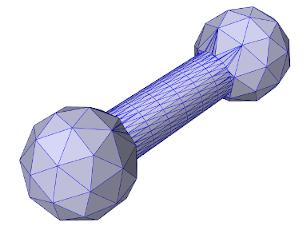
\includegraphics[]{images/dumbbellMeshUnion}
\else
 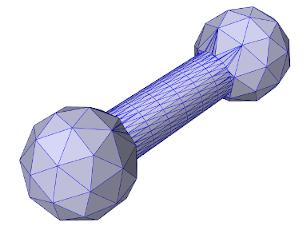
\includegraphics[width=3in]{images/dumbbellMeshUnion}
\fi
\end{center}
\caption{Dumbbell shaped mesh produced from the CSG union of
two balls and a cylinder.}
\label{dumbbellMeshUnion:fig}
\end{figure}

The CSG operations include union, intersection, and difference, and
are implemented by the following methods of {\tt SurfaceMeshIntersector}:
% method table
\begin{lstlisting}[]
  findUnion (mesh0, mesh1);         // volume0 U volume1
  findIntersection (mesh0, mesh1);  // volume0 ^ volume1
  findDifference01 (mesh0, mesh1);  // volume0 - volume1 
  findDifference10 (mesh0, mesh1);  // volume1 - volume0 
\end{lstlisting}
%
Each takes two {\tt PolyhedralMesh} objects, {\tt mesh0} and {\tt
mesh1}, and creates and returns another {\tt PolyhedralMesh} which
represents the boundary surface of the requested operation. If the
result of the operation is {\tt null}, the returned mesh will be empty.

The example below uses {\tt findUnion} to create a dumbbell shaped mesh
from two balls and a cylinder:
%
\begin{lstlisting}[]
  // first create two ball meshes and a bar mesh
  double radius = 1.0;
  int division = 1; // number of divisons for icosahedral sphere
  PolygonalMesh ball0 = MeshFactory.createIcosahedralSphere (radius, division);
  ball0.transform (new RigidTransform3d (0, -2*radius, 0));
  PolygonalMesh ball1 = MeshFactory.createIcosahedralSphere (radius, division);
  ball1.transform (new RigidTransform3d (0, 2*radius, 0));
  PolygonalMesh bar = MeshFactory.createCylinder (
     radius/2, radius*4, /*ns=*/32, /*nr=*/1, /*nh*/10);
  bar.transform (new RigidTransform3d (0, 0, 0, 0, 0, Math.PI/2));

  // use a SurfaceMeshIntersector to create a CSG union of these meshes
  SurfaceMeshIntersector smi = new SurfaceMeshIntersector();
  PolygonalMesh balls = smi.findUnion (ball0, ball1);
  PolygonalMesh mesh = smi.findUnion (balls, bar);
\end{lstlisting}
%
The balls and cylinder are created using the
\javaclass[\mgeo]{MeshFactory} methods
\javamethod*[\mgeo.MeshFactory]{createIcosahedralSphere(double,int)}
and
\javamethod*[\mgeo.MeshFactory]{createCylinder(double,double,int,int,int)},
where the latter takes arguments {\tt ns}, {\tt nr}, and {\tt nh}
giving the number of slices along the circumference, end-cap radius,
and length. The final resulting mesh is shown in Figure
\ref{dumbbellMeshUnion:fig}.

%\section{Geometric Queries}
%\label{GeometricQueries:sec}
%
%XXX

\section{Reading source relative files}
\label{PathFinder:sec}

ArtiSynth applications frequently need to read in various kinds of
data files, including mesh files (as discussed in Section
\ref{MeshFileIO:sec}), FEM mesh geometry (Section
\ref{FemGeometryFiles:sec}), probe data (Section
\ref{DataFileFormat:sec}), and custom application data.

Often these data files do not reside in an absolute location but
instead in a location relative to the application's class or source
files.  For example, it is common for applications to store geometric
data in a subdirectory {\tt "geometry"} located beneath the source
directory. In order to access such files in a robust way, and ensure
that the code does not break when the source tree is moved, it is
useful to determine the application's source (or class) directory at
run time. ArtiSynth supplies several ways to conveniently handle this
situation. First, the {\tt RootModel} itself supplies the following
methods:
% method table
\begin{lstlisting}[]
  // find path to the root model's source directory
  String findSourceDir ();

  // get path to a file specified relative to the root model's source directory
  String getSourceRelativePath (String relpath);
\end{lstlisting}
%
The first method returns the path to the source directory of the
root model, while the second returns the path to a file specified
relative to the root model source directory. If the root model source
directory cannot be found (see discussion at the end of this section)
both methods return {\tt null}.
%
As a specific usage example, assume that we have an application model
whose {\tt build()} method needs to load in a mesh {\tt torus.obj}
from a subdirectory {\tt meshes} located beneath the source
directory. This could be done as follows:
%
\begin{lstlisting}[]
  String pathToMesh = getSourceRelativePath ("meshes/torus.obj");
  // read the mesh from a .obj file :
  WavefrontReader reader = new WavefrontReader (pathToMesh);
  PolygonalMesh mesh = null;
  try {
     mesh = reader.readMesh () ;
  }
  catch (IOException e) {
     System.err.println ("Can't read mesh:");
     e.printStackTrace () ;
  }
\end{lstlisting}

A more general path finding utility is provided by
\javaclass{maspack.util.PathFinder}, which provides several static
methods for locating source and class directories:
% method table
\begin{lstlisting}[]
  // find path to the source directory associated with classObj
  String findSourceDir (Object classObj);

  // get path to a file specified relative to classObj source directory
  String getSourceRelativePath (Object classObj, String relpath);

  // find path to the class directory associated with classObj
  String findClassDir (Object classObj);

  // get path to a file specified relative to classObj class directory
  String getClassRelativePath (Object classObj, String relpath);
\end{lstlisting}
%
The ``find'' methods return a string path to the indicated class or
source directory, while the ``relative path'' methods locate the class
or source directory and append
the additional path {\tt relpath}.  For all of these, the class is
determined from {\tt classObj}, either directly (if it is an instance
of {\tt Class}), by name (if it is a {\tt String}), or otherwise by
calling {\tt classObj.getClass()}. When identifying a package by name,
the name should be either a fully qualified class name, or a simple
name that can be located with respect to the packages obtained via
{\tt Package.getPackages()}. For example, if we have a class whose
fully qualified name is {\tt artisynth.models.test.Foo}, then the
following calls should all return the same result:
%
\begin{lstlisting}[]
   Foo foo = new Foo();

   PathFinder.findSourceDir (foo);
   PathFinder.findSourceDir (Foo.class);
   PathFinder.findSourceDir ("artisynth.models.test.Foo");
   PathFinder.findSourceDir ("Foo");
\end{lstlisting}
%
If the source directory for {\tt Foo} happens to be {\tt
/home/projects/src/artisynth/models/test}, then
%
\begin{lstlisting}[]
   PathFinder.getSourceRelativePath (foo, "geometry/mesh.obj");
\end{lstlisting}
%
will return
{\tt /home/projects/src/artisynth/models/test/geometry/mesh.obj}.

\begin{sideblock}
When calling {\tt PathFinder} methods from {\it within} the relevant
class, one can specify {\tt this} as the {\tt classObj} argument.
\end{sideblock}

With respect to the above example locating the file {\tt
"meshes/torus.obj"}, the call to the root model method 
{\tt getSourceRelativePath()} could be replaced with
%
\begin{lstlisting}[]
  String pathToMesh = PathFinder.getSourceRelativePath (
     this, "meshes/torus.obj");
\end{lstlisting}
Since this is assumed to be called from the root model's build method,
the ``class'' can be indicated by simply passing {\tt this} to {\tt
getSourceRelativePath()}.

\begin{sideblock}
As an alternative to placing data files in the source directory, one
could place them in the class directory, and then use {\tt
findClassDir()} and {\tt getClassRelativePath()}. If the data files
were originally defined in the source directory, it will be necessary
to copy them to the class directory. Some Java IDEs will perform this
automatically.
\end{sideblock}

The {\tt PathFinder} methods work by climbing the class's resource
hierarchy.  Source directories are assumed to be located relative to
the parent of the root class directory, via one of the paths specified
by \javamethod[maspack.util.PathFinder]{getSourceRootPaths()}. By default, this
list includes {\tt "src"}, {\tt "source"}, and {\tt "bin"}. Additional
paths can be added using
\javamethodAlt{maspack.util.PathFinder.addSourceRootPath()}%
{addSourceRootPath(path)},
or the entire list can be set using
\javamethodAlt{maspack.util.PathFinder.setSourceRootPaths()}%
{setSourceRootPaths(paths)}.

At preset, source directories will not be found if the reference class
is contained in a jar file.

\section{Reading and caching remote files}
\label{FileManager:sec}

ArtiSynth applications often require the use of large data files to
specify items such as FEM mesh geometry, surface mesh geometry, or
medical imaging data. The size of these files may make it inconvenient
to store them in any version control system that is used to
store the application source code. As an alternative, ArtiSynth
provides a {\it file manager} utility that allows such files to be
stored on a separate server, and then downloaded on-demand and cached
locally. To use this, one starts by creating an instance of a
\javaclass[maspack.fileutil]{FileManager}, using the constructor
% method def
\begin{lstlisting}[]
  FileManager (String downloadPath, String remoteSourceName)
\end{lstlisting}
%
where {\tt downloadPath} is a path to the local directory where the
downloaded file should be placed, and {\tt remoteSourceName} is a URI
indicating the remote server location of the files.  After the file
manager has been created, it can be used to fetch remote files and
cache them locally, using various {\it get} methods:
% methd table
\begin{lstlisting}[]
  File get (String destName);

  File get (String destName, String sourceName);
\end{lstlisting}
%
Both of these look for the file {\tt destName} specified relative to
the local directory, and return a {\tt File} handle for it if it is
present. Otherwise, they attempt to download the file from the remote
source location, place it in the local directory, and return a {\tt
File} handle for it.
The location of the remote file is given relative to
the remote source URI by {\tt destName} for the first method and {\tt
sourceName} for the second.

A simple example of using a file manager within a {\tt RootModel} {\tt
build()} method is given by the following fragment:
%
\begin{lstlisting}[]
  // create the file manager ...
  FileManager fm = new FileManager (
    getSourceRelativePath("geometry"), 
    "http://myserver.org/artisynth/data/geometry");
  // ... and use it to get a bone mesh file
  File meshFile = fm.get ("tibia.obj");
\end{lstlisting}
%
Here, a file manager is created that uses a local directory {\tt "geometry"},
located relative to the {\tt RootModel} source directory (see Section
\ref{PathFinder:sec}), and looks for missing files relative to the URI
%
\begin{verbatim}
  http://myserver.org/artisynth/data/geometry
\end{verbatim}
%
The {\tt get()} method is then used to obtain the file {\tt
"tibia.obj"} from the local directory. If it is not already present,
it is downloaded from the remote location.

The \javaclass[maspack.fileutil]{FileManager} contains other features
and functionality, and one should consult its API documentation for
more information.

\ifdefined\maindoc
\else
\end{document}
\fi
